\begin{figure}[ht!]
\centering
% \caption{}
% % 
% % 
% % Dominator analysis performs traversal over the graph to determine the
% % dominators of each node. It has two traversals. \textit{init} traversal collects
% % all node ids. \textit{dom\_T} is called with a fixpoint and it runs till all the
% % nodes reach the fixpoint condition.}
% \label{fig:dominator}
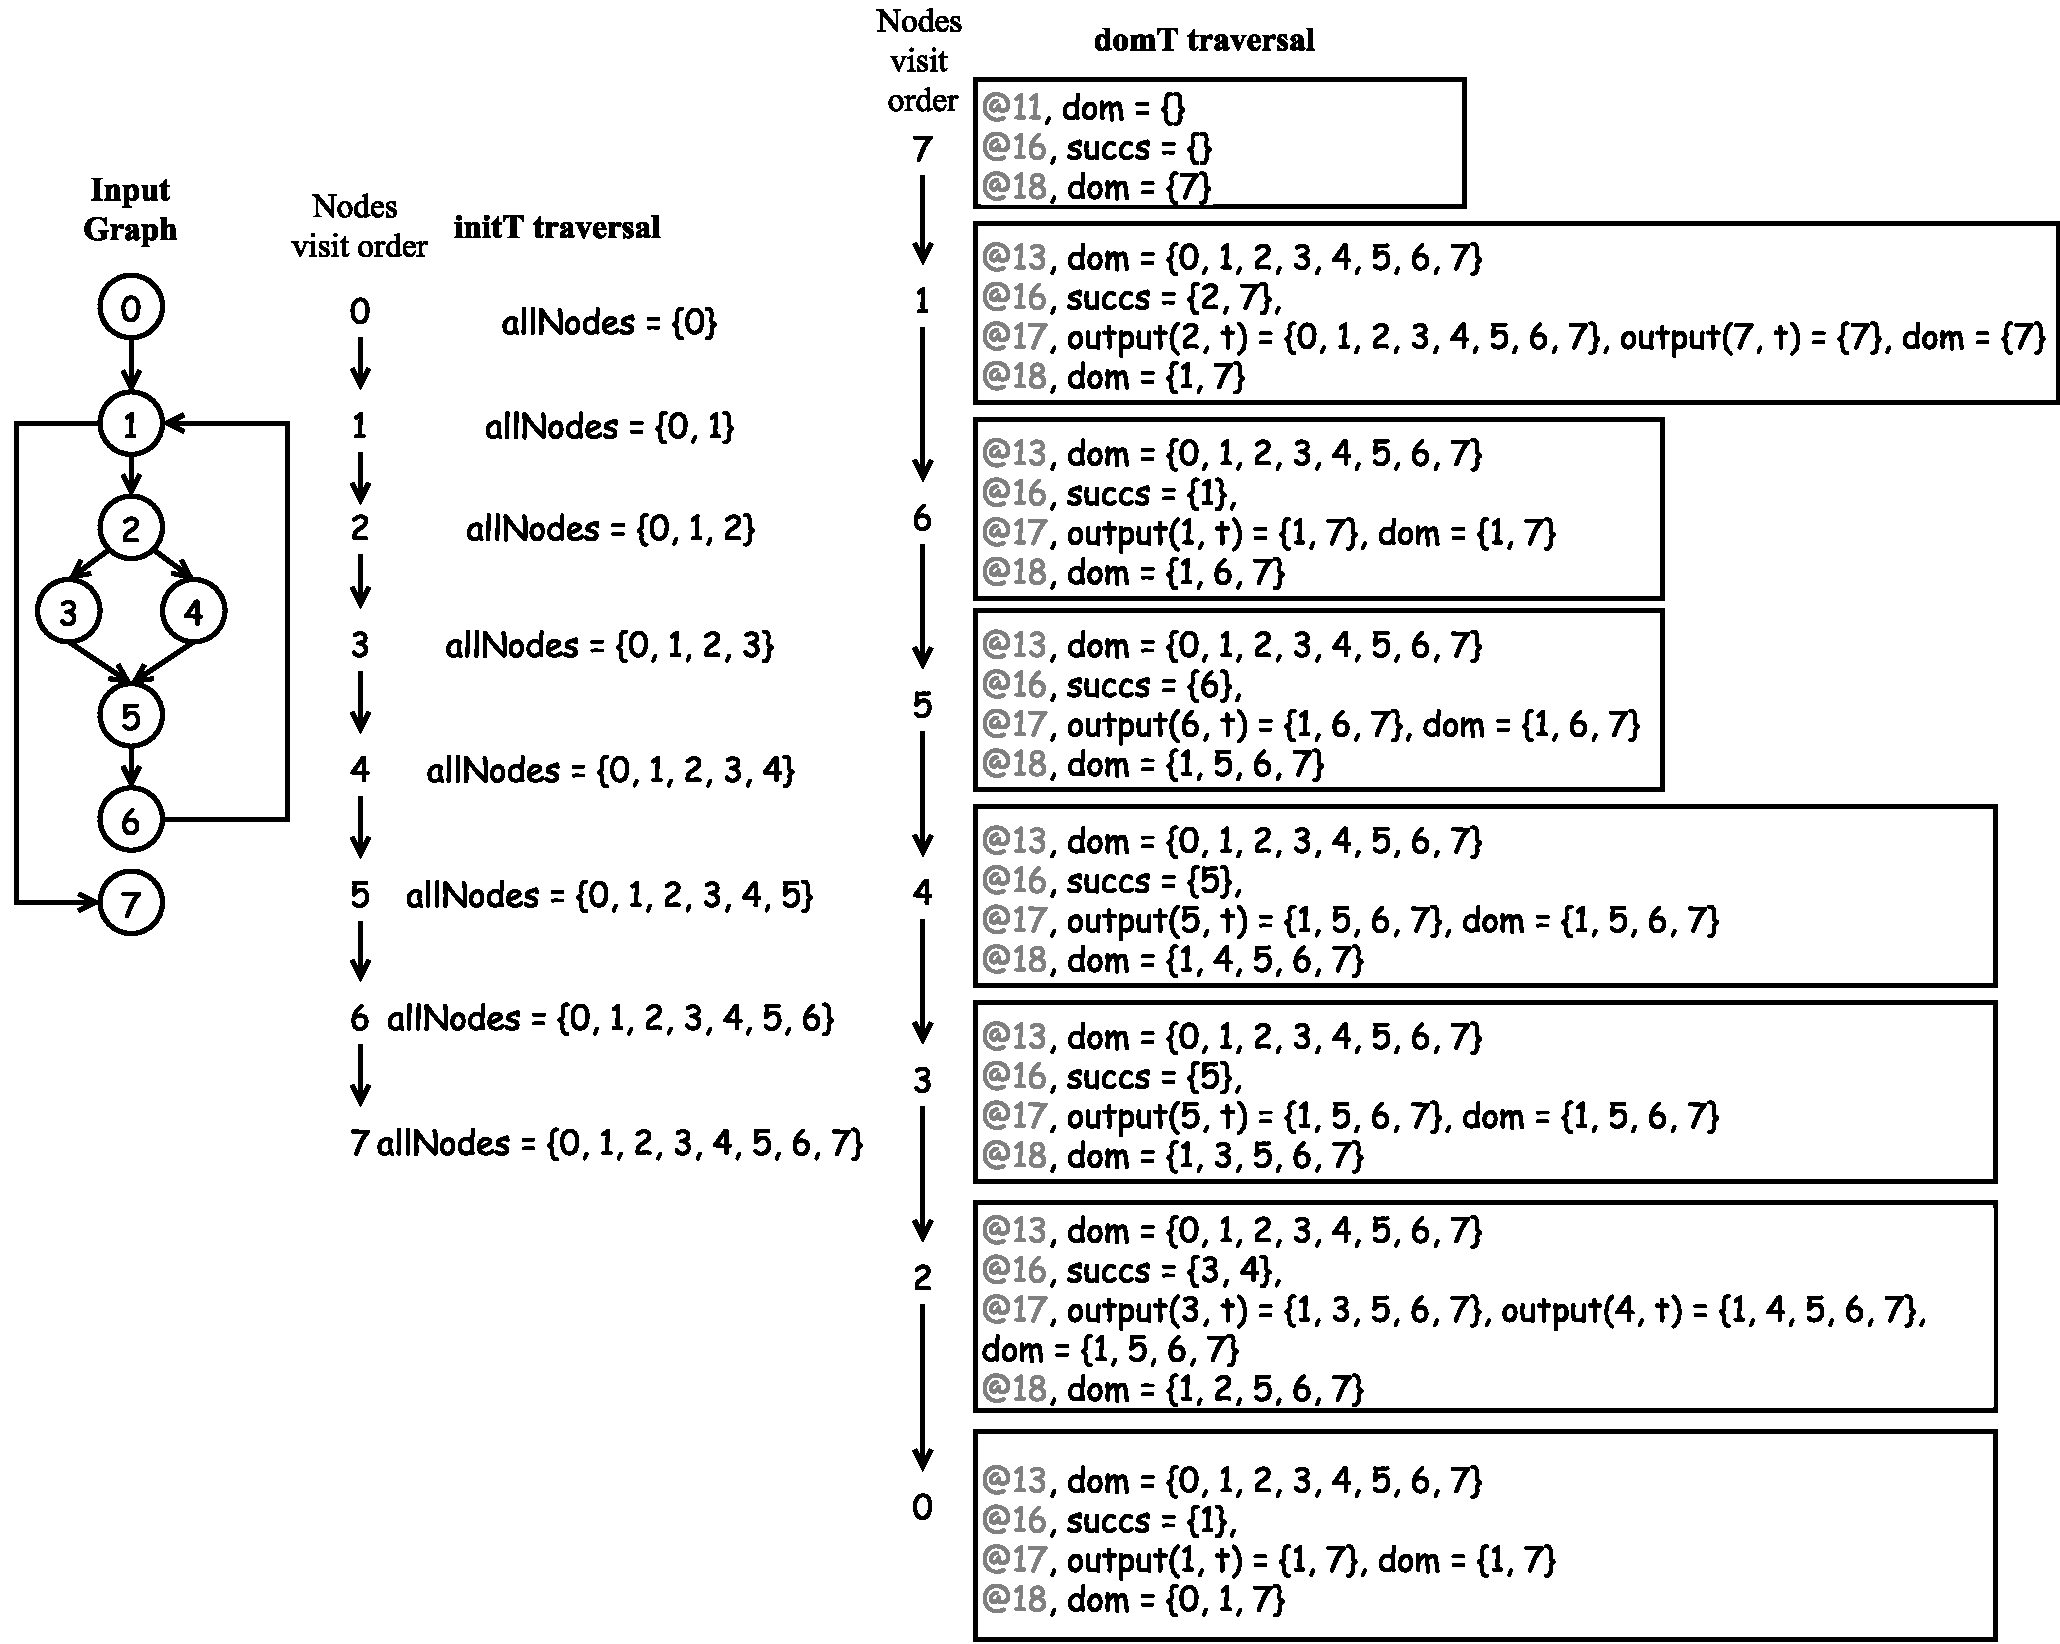
\includegraphics[width=0.9\linewidth]{figures/running-example.pdf}
\caption{Running example of applying the post dominator analysis on an input
graph containing branch and loop.}
\label{fig:running-example}
\end{figure}


